\chapter{کارهای پیشین}
\pagebreak
\section{‌مقدمه}
در دو فصل گذشته، مسئله‌ی درک زبان طبیعی تعریف شده و پایه‌های سازنده‌ی آن معرفی شدند. سپس مفاهیم پایه که برای فهم موضوع لازم بود ذکر شده و در ادامه، ساختار شبکه‌های عصبی گوناگون، که در حل مسئله‌ی درک زبان استفاده می‌شوند، تشریح شدند. برای بستر سازی لازم جهت معرفی مدل، لازم است کارهای پیشین معرفی شوند تا تلاش‌هایی که تا کنون برای بهبود دو وظیفه‌ی تشخیص هدف و پر کردن جای خالی صورت گرفته است، هویدا شود. بر این اساس، در فصل پیش رو، تحقیقات پیشین در این زمینه و مدل‌های ارائه شده توصیف می‌شوند. از آنجا که روش‌های ارائه شده با یکدیگر متفاوت بوده و اشتراکات اندکی دارند، دسته‌بندی آن‌ها به دسته‌های معنادار، کار دشواری است. در فصل پیش رو،  مدل‌های ارائه شده بر پایه‌ی سبک تعبیه و اساس معماری شبکه تقسیم بندی می‌شوند.


در گذشته، دو وظیفه‌ی پر کردن جای خالی و تشخیص هدف جداگانه مورد تحقیق قرار می‌گرفتند \cite{louvan2018exploring,vu2016bi}؛ اما اخیراً، نشان داده شده که آموزش مشترک این دو وظیفه، اثر مثبتی بر عملکرد هر دوی آن‌ها دارد
\cite{aligned_lstm_atten_nlu,Wang:18,goo-etal-2018-slot,zhang-2018-joint,jaech2016domain,wei2022joint}.
این امر نشان داده است که رابطه‌ای قوی بین این دو وجود دارد. آموزش همزمان این دو وظیفه به این صورت انجام می‌گیرد که برای هر دوی آن‌ها یک رمزنگار مشترک استفاده شده، اما برای هر وظیفه یک رمزگشای مستقل تعریف می‌شود. تمامی مدل‌هایی که در این زمینه‌ی درک زبان طبیعی وجود دارند، از این ساختار بهره می‌برند چراکه برتری آن ثابت شده است.
\section{مبتنی بر نمایش تعبیه برداری ثابت}

مدت‌ها است که مکانیزم توجه به همراه \lr{LSTM‌} مورد استفاده قرار می‌گیرد \cite{varghese2020bidirectional,jaech2016domain}. ترکیب این دو در وظیفه‌ی درک زبان طبیعی نیز مورد استفاده قرار گرفته و در زمان خود بهترین عملکرد را در پی داشت. از طرفی، به علت رابطه‌ی یک به یک واژه‌های ورودی به برچسب‌های خروجی، نیازی به فضای باز احتمالاتی خروجی یک \lr{LSTM‌} نبود. به عبارت دیگر، نیاز نبود طول جمله‌ی خروجی پویا باشد؛ بلکه خروجی با طول ثابت و هم اندازه با ورودی مورد انتظار است. از طرف دیگر، آگاهی از اینکه کدام موقعیت از ورودی، به خروجی مربوط است، خود یک مزیت محسوب می‌شود و باید از آن در طراحی معماری شبکه استفاده کرد \cite{xu2020end}. در طراحی مدل \lr{LSTM}‌ تراز شده، از رابطه‌ی یک به یک ورودی با خروجی بهره برده شد \cite{aligned_lstm_atten_nlu}. شکل \ref{Fig:alignedlstm} معماری مدل تراز شده را نمایش می‌دهد. در این معماری، برای رمزنگار، از یک \lr{LSTM‌} دوطرفه که به صورت مشترک در دو رمزگشا مورد بهره‌وری قرار می‌گرفت. در رمزگشای تشخیص هدف، از بردار توجه هدف، و همچنین آخرین حالت مخفی \lr{LSTM‌} رمزنگار برای کلاس بندی اهداف بهره برده شده بود. اما در رمزگشای پر کردن جای خالی، یک \lr{LSTM‌} یک طرفه تعریف شده و از رابطه‌ی یک به یک ورودی و خروجی استفاده شد. به این منظور، در هر گام زمانی، علاوه بر بردار توجه، بردار حالت مخفی مربوط به گام زمانی ورودی که متناظر با گام زمانی خروجی بود، به مدل تغذیه می‌شد. با این ترتیب از ورودی‌ها، آموزش دو وظیفه‌ی تشخیص هدف و پر کردن جای خالی، به صورت همزمان و اشتراک آن ازطریق مشترک بودن تابع خطای آن دو وظیفه بود.
\begin{figure}[!htb]
	\centering
	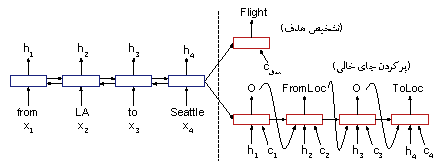
\includegraphics[scale=1.6]{Figures/alignedcnnblstm.pdf}
	\caption[ساختار مدل \lr{Aligned BLSTM}]{ساختار مدل \lr{Aligned BLSTM} \cite{aligned_lstm_atten_nlu}.}
	\label{Fig:alignedlstm}
\end{figure}


در پژوهشی دیگر، با ترکیب معماری \lr{LSTM‌} تراز شده با شبکه‌ی عصبی کانولوشنی و ساختار توالی ویژگی پنجره، نتایج بهتری به دست آمد \cite{Wang:18}. در این شبکه که آن را \lr{Aligned CNN-BLSTM} نامیدند، در بخش رمزنگار، عملیات کانولوشن با اندازه هسته‌های مختلف صورت گرفته، و نتیجه‌ی حاصل پس از ترانهاده شدن، به یکدیگر الحاق می‌شد. این ساختار را توالی ویژگی پنجره نامیدند. سپس خروجی این ساختار به یک \lr{LSTM‌} دوطرفه برای تعبیه داده می‌شد. رمزگشای پیشنهادی این مدل در هر دو وظیفه، با \lr{Aligned BLSTM} یکسان در نظر گرفته شد. شکل \ref{Fig:wang18} ساختار این شبکه را نمایش می‌دهد. این ساختار به عنوان پایه‌ی کار \lr{CTran} درنظر گرفته شد؛ از این رو در بخش ۴، شباهت زیادی میان ساختار رمزنگار پیشنهادی و این مدل خواهید دید. بخش رمزنگار این شبکه نیز کاملا با شبکه‌ی \cite{aligned_lstm_atten_nlu} یکسان بود. متعاقباً، اشتراک آموزش دو وظیفه نیز با اشتراک گذاری تابع خطا اتفاق می‌افتاد.
\begin{figure}[!htb]
	\centering
	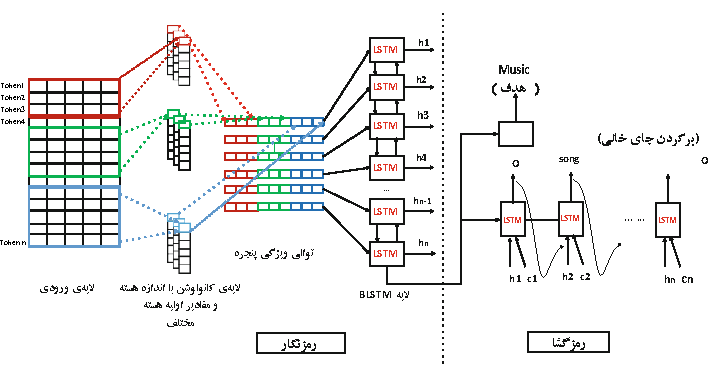
\includegraphics[scale=1.1]{Figures/cnnblstm.pdf}
	\caption[ساختار مدل \lr{Aligned CNN-BLSTM}]{ساختار مدل \lr{Aligned CNN-BLSTM} \cite{Wang:18}.}
	\label{Fig:wang18}
\end{figure}


اما در مدل \lr{Slot-Gated} \cite{goo-etal-2018-slot}، علاوه بر آموزش مشترک دو وظیفه از طریق اشتراک تابع خطا، با به اشتراک گذاری بردارهای توجه نیز اطلاعات وظیفه‌ی تشخیص هدف را در اختیار وظیفه‌ی پر کردن جای خالی گذاشتند. در معماری \lr{Slot-Gated} که در شکل \ref{Fig:slotgate} ترسیم شده، از یک شبکه‌ی \lr{LSTM‌} دوطرفه برای تعبیه‌ی جمله‌ی ورودی استفاده شد. این \lr{LSTM‌} میان هر دو وظیفه مشترکاً و به عنوان رمزنگار مدل به کار گرفته شد. سپس در رمزگشا، مکانیزم توجه \cite{attention_bahdanau} برای هر وظیفه به صورت جداگانه روی آن لایه‌ی \lr{LSTM‌} اعمال گردید. برای تولید احتمالات تشخیص هدف، آخرین خروجی \lr{LSTM‌} همراه با بردار توجه\RTLfootnote{ لازم به ذکر است که معمولا مکانیزم توجه از یک ماتریس $\mathbb{R}^{i\times j}$ تشکیل شده که در آن $i$ به عنوان طول جمله مبدا و $j$ طول جمله‌ی مقصد است؛ اما چون در تشخیص هدف تنها یک مقصد وجود دارد، یک بردار $\mathbb{R}^{i}$ تولید می‌شود.} جمع شده، سپس به یک لایه‌ی تماماً متصل تغذیه شد و با استفاده از سافت‌مکس، احتمالات خروجی برای تشخیص هدف به دست آمد.  اما برای وظیفه‌ی پر کردن جای خالی، یک دروازه‌ی جدید معرفی شد. این دروازه درواقع یک امتیاز بود که در بردار توجه جای خالی ضرب می‌شد. نتیجه‌ی ضرب، با بردار حالت مخفی برای هر مرحله از تولید برچسب جمع می‌شد و سپس بردار نهائی بدست آمده با استفاده از یک لایه‌ی تماما متصل و سافت‌مکس، احتمالات خروجی را تولید می‌کرد. به عبارتی، در معماری مدل \lr{Slot-Gated}، هیچ شبکه‌ی بازگشتی در رمزگشا استفاده نشد. امتیاز ذکر شده، از جمع وزن‌دار بردار توجه تشخیص هدف، که در بعد زمانی گسترده شده بود، با بردار توجه جای خالی بدست می‌آمد. 
\begin{figure}[!htb]
	\centering
	\includegraphics[scale=1.3]{Figures/slotgate.pdf}
	\caption[ساختار مدل \lr{Slot-Gate}]{ساختار مدل \lr{Slot-Gate} \cite{goo-etal-2018-slot}.}
	\label{Fig:slotgate}
\end{figure}


در روش \lr{Slot-Gate}، اطلاعات برچسب‌های تولید شده در تشخیص هدف مورد بهره‌وری واقع نمی‌شد؛ از این رو، ارتباطات مستقیم دوطرفه برقرار نمی‌گردید. مدل \lr{Inter-Related} \cite{e:2019} که در شکل \ref{Fig:interrelated} ترسیم شده، شبکه‌ی \lr{SF-ID} را معرفی کرد که از یک زیر شبکه‌ی پر کردن جای خالی و یک زیر شبکه‌ی تشخیص هدف ساخته می‌شد. زیر شبکه‌ی پر کردن جای خالی، اطلاعات تشخیص هدف را وارد پر کردن جای خالی کرده و در مقابل، زیر شبکه‌ی تشخیص هدف، اطلاعات برچسب‌های تولید شده را بر شبکه‌ی تشخیص هدف اعمال می‌کرد. اما برای تولید هرکدام، نیاز به داشتن دیگری است. از این رو، این مدل، مکانیزم تکرار را معرفی کرد که در آن، یک وظیفه به عنوان نقطه‌ی آغاز انتخاب می‌شد، اما فرایند انتخاب تا تعداد دفعه‌ی مشخصی تکرار می‌شد. به این ترتیب اطلاعات معنایی هر دو وظیفه می‌توانستند با یکدیگر ترکیب شوند. ازنظر ساختار شبکه‌ای، این مدل در رمزنگار خود یک \lr{LSTM‌} دوطرفه را به صورت مشترک برای دو وظیفه استفاده می‌کند. سپس در این مدل، مکانیزم توجه جداگانه برای هر وظیفه تعریف می‌شود. در رمزگشای آن، مکانیزم تکرار ابداعی قرار گرفته است. در پایان، برای تولید احتمالات هدف از لایه‌ی تماماً متصل، و برای تولید برچسب از \lr{CRF} استفاده گردیده است.
\begin{figure}[!htb]
	\centering
	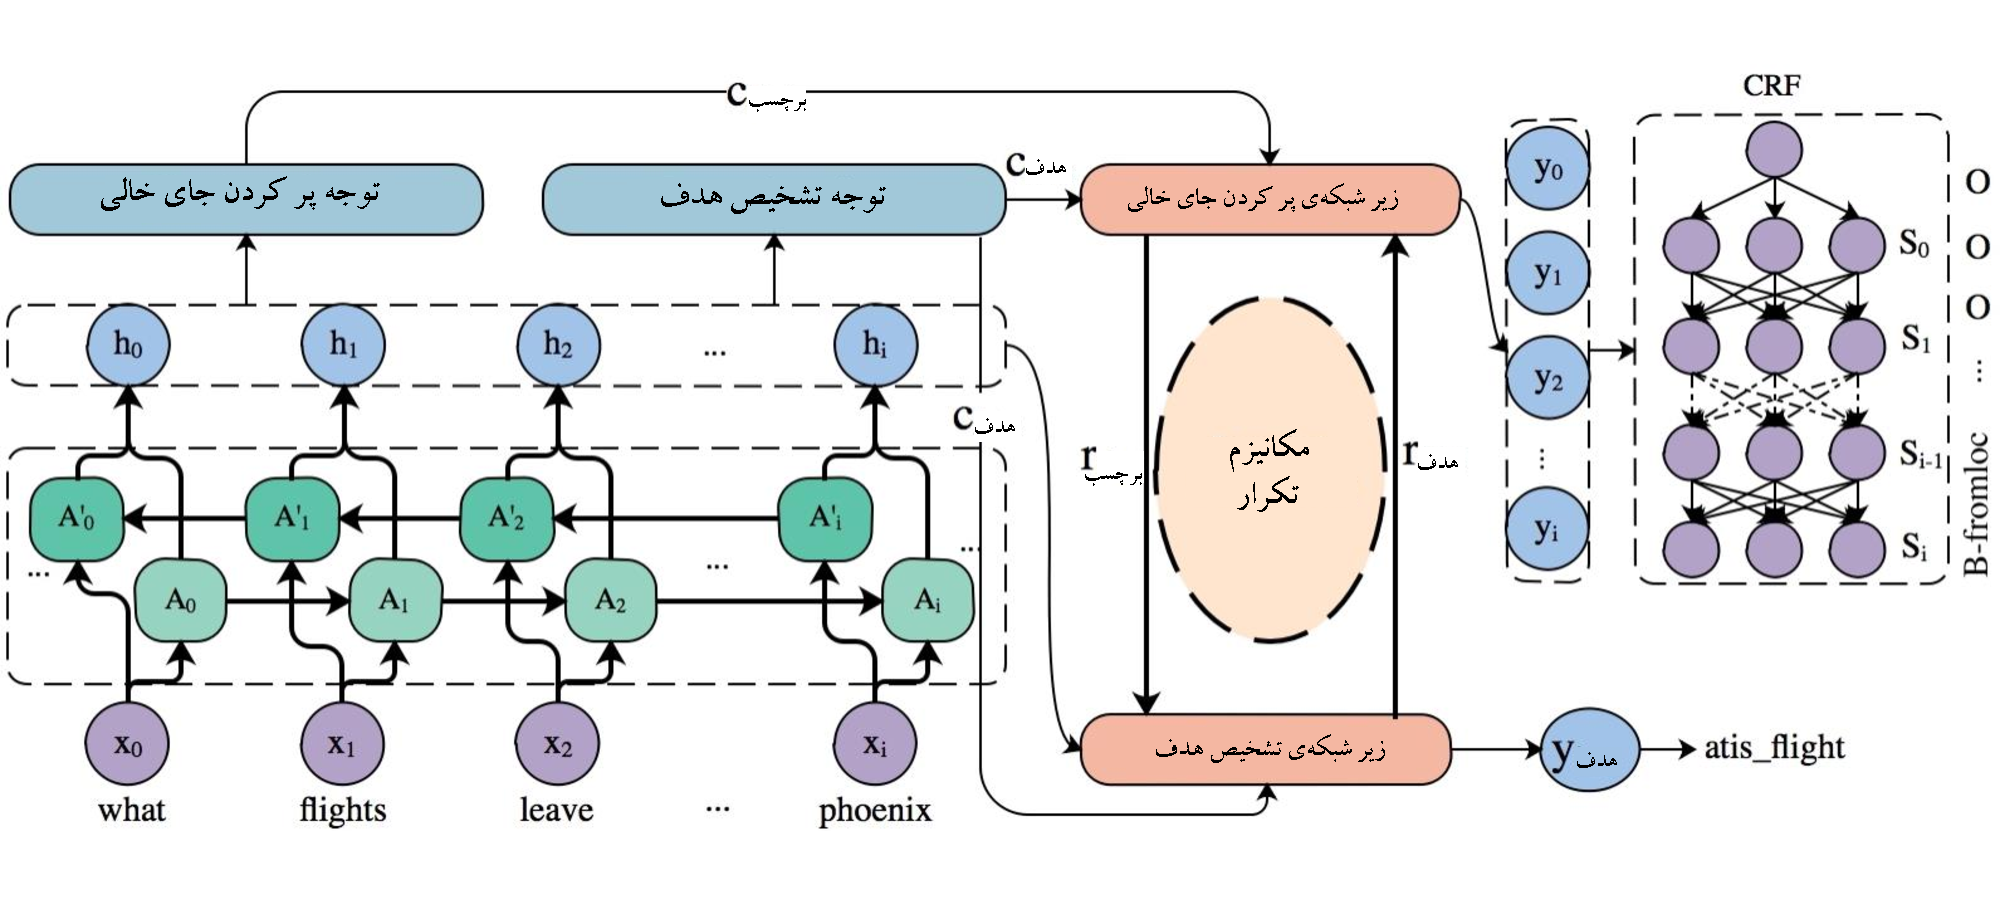
\includegraphics[scale=0.45]{Figures/interrelated.pdf}
	\caption[ساختار مدل \lr{Inter-Related}]{ساختار مدل \lr{Inter-Related} \cite{e:2019}.}
	\label{Fig:interrelated}
\end{figure}


در \lr{CharEmbed+GRU}\ \cite{Firdaus:2021} تعبیه‌ی سطح الفبا برای درک زبان طبیعی پیشنهاد شد. به این منظور، ابتدا کلمات را به الفبای سازنده شکسته، و حروف الفبای واژه را به یک \lr{LSTM‌} دوطرفه دادند تا تعبیه‌ی سطح الفبای دوطرفه ایجاد شود. در پایان، از الحاق تعبیه‌ی ایجاد شده از \lr{LSTM‌} با یک تعبیه‌ی سطح واژه مانند \lr{Word2Vec}، تعبیه‌ی نهائی واژه را ساختند. در معماری این مدل، از \lr{LSTM‌} دو طرفه برای رمزنگار و از \lr{CRF} برای رمزگشا استفاده شد.
شکل \ref{Fig:firdaus} نشان دهنده‌ی معماری \lr{CharEmbed+GRU} است که شیوه‌ی جدیدی برای ایجاد تعبیه‌ی واژه‌ها ایجاد کرد \cite{Firdaus:2021}. این مدل با قراردادن شبکه‌ی کانولوشنی بر روی الفبای کلمات و سپس عملیات \lr{Max-Pooling}، یک تعبیه‌ی سطح الفبا برای واژه ایجاد کرد. سپس تعبیه‌ی سطح الفبا را با تعبیه‌ی واژه‌ی مورد پردازش، الحاق کرد. حاصل این الحاق، به عنوان تعبیه‌ی یک واژه در نظر گرفته شد. این تعبیه برای تمام واژه‌های جمله ایجاد شده و وارد پشته‌ی \lr{LSTM} گردید تا یک تعبیه برای جمله ایجاد شود. سپس با استفاده از مکانیزم توجه \cite{attention_bahdanau} و تغذیه‌ی آن به یک لایه‌ی خطی و سافت مکس، احتمالات خروجی تشخیص هدف، پر کردن جای خالی و طبقه بندی قانون گفتگو\LTRfootnote{Dialogue Act Classification} تولید شد.
\begin{figure}[!htb]
	\centering
	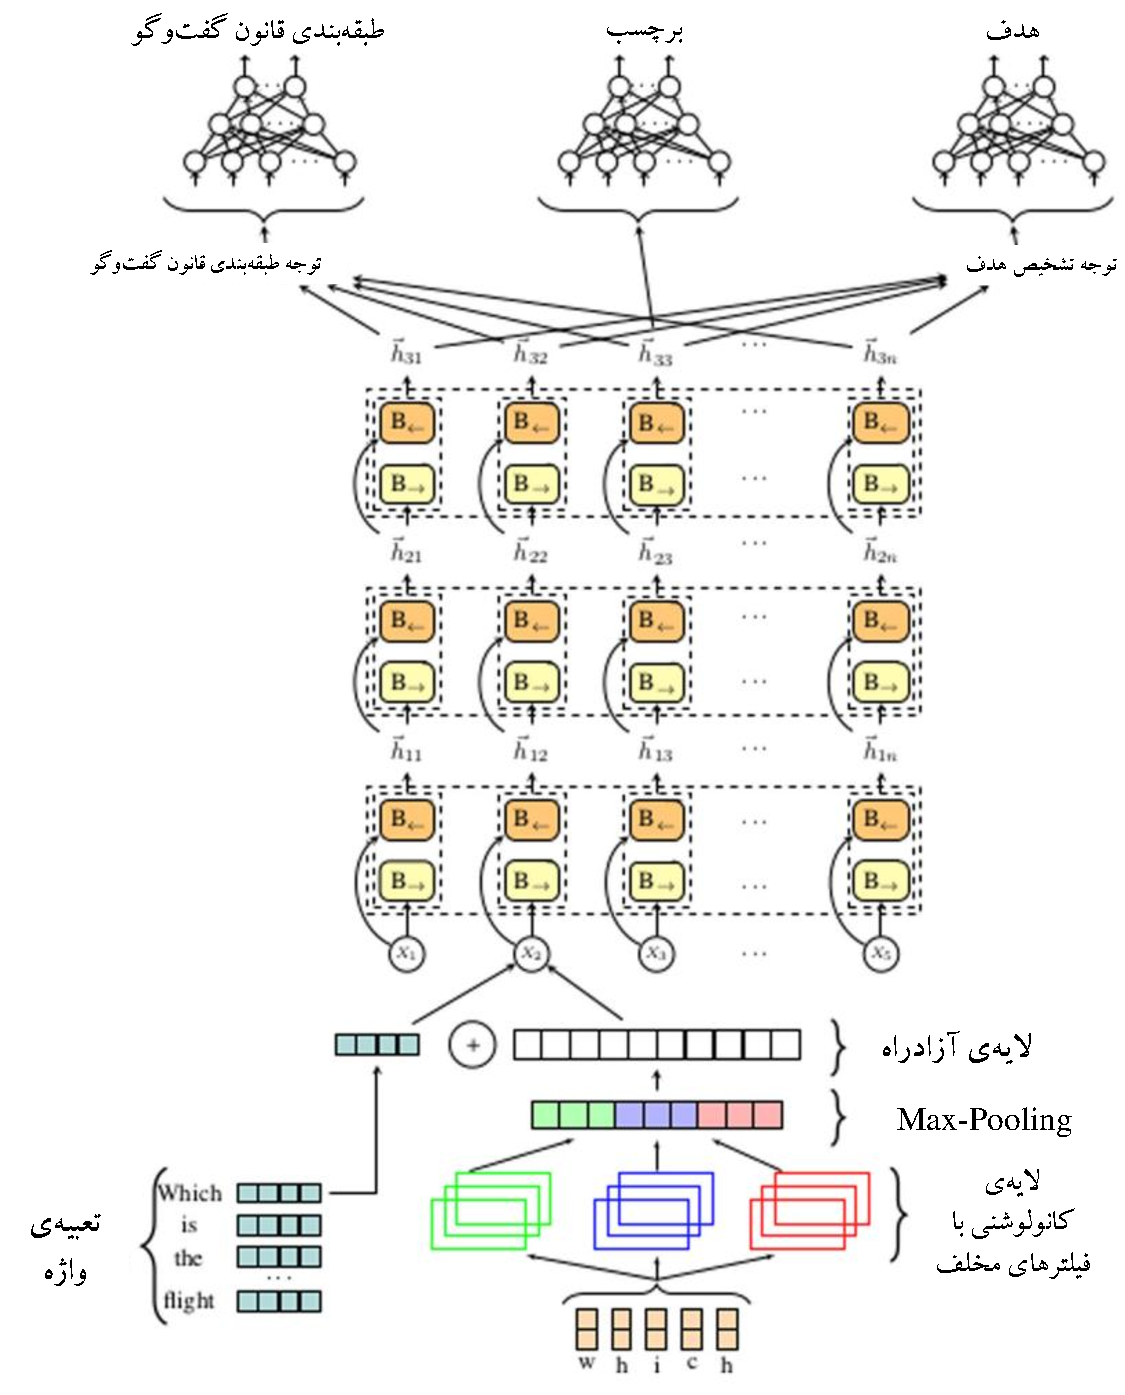
\includegraphics[scale=0.6]{Figures/firdaus2021.pdf}
	\caption[ساختار مدل پیشنهادی \lr{CharEmbed+GRU}]{ساختار مدل پیشنهادی \lr{CharEmbed+GRU} \cite{Firdaus:2021}.}
	\label{Fig:firdaus}
\end{figure}


مدل \lr{PKJL}\LTRfootnote{Prior Knowledge Joint Learning}  برای افزایش به اشتراک گذاری اطلاعات قبلی با دو وظیفه‌ی پر کردن جای خالی و تشخیص هدف معرفی شد \cite{priorknowledge}. منظور از اطلاعات قبلی، احتمال وقوع هر برچسب هدف با هر برچسب جای خالی در یک نمونه‌ی آموزشی است. در معماری پیشنهادی \lr{PKJL} که در شکل \ref{Fig:model_pkjl} ترسیم شده، مدل \lr{PKJL} با محاسبه‌ی این احتمالات و تغذیه‌ی آن به مدل خود در یک لایه‌ی ابداعی، دانش قبلی را با مدل به اشتراک گذاشت. معماری این مدل که در شکل \ref{Fig:model_pkjl}  به تصویر کشیده شده است، از یک \lr{LSTM} دو طرفه در رمزنگار و بردار احتمالات وقوع هر برچسب با هر هدف تشکیل می‌شد. یک ماژول ابداعی به نام لایه‌ی یکپارچه سازی اطلاعات بعد از رمزنگار ایجاد شد که سه ماتریس توجه برای تشخیص هدف، پر کردن جای خالی و دانش قبلی در آن تعریف می‌شدند. این سه ماتریس با یکدیگر تجمیع و تبدیل خطی شدند تا خروجی ماژول ابداعی تکمیل شود. در رمزگشای پر کردن جای خالی، یک \lr{CRF} و در رمزنگار تشخیص هدف، یک لایه‌ی خطی همراه با سافت‌مکس استفاده شد.
\begin{figure}[!htb]
	\centering
	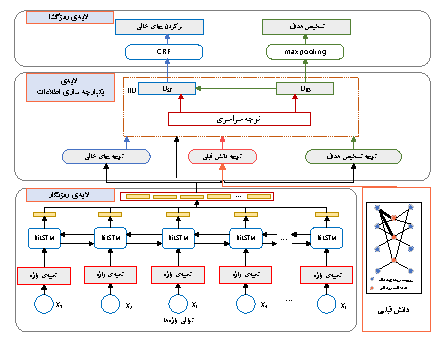
\includegraphics[scale=2]{Figures/priorknowledge.pdf}
	\caption[ساختار مدل \lr{PKJL}]{ساختار مدل \lr{PKJL} \cite{priorknowledge}.}
	\label{Fig:model_pkjl}
\end{figure}
\section{مبتنی بر مدل زبانی به عنوان رمزنگار}
طراحی مدل زبانی برت به نحوی است که استفاده از آن در وظایف مختلف پردازش زبان طبیعی بسیار ساده است. در مدل پایه که توسط \cite{chen:2019} معرفی شد، یک لایه‌ی تماماً متصل بر روی هریک از خروجی‌های برت قرار گرفت تا خروجی آن که به بعد آن، همان ابعاد تعبیه‌ی است، تبدیل به تعداد کلاس‌های برچسب‌ها و هدف‌های مجموعه داده شود. بدین ترتیب، خروجی نشانه‌ی $[CLS]$ برای مشخص کردن هدف کاربر، و نشانه‌های بخش اول ورودی به عنوان نتیجه‌ی برچسب‌زنی در نظر گرفته شد. بدین ترتیب، رمزنگار شبکه خود مدل برت و رمزگشا یک لایه‌ی تماماً متصل در نظر گرفته شد.
در معماری \cite{chen:2019}، از برت به عنوان رمزنگار استفاده شد. اما برت در درک روابط منطقی میان برچسب‌های هدف، خوب عمل نمی‌کند و این مشکل باعث می‌شود عملکرد پر کردن جای خالی شدیداً تحت تاثیر قرار گیرد \cite{Wang:2020}. از این رو، مدل \lr{SASGBC} \cite{Wang:2020} معرفی شد، که حاوی دو راهکار برای مقابله با مشکل ذکر شده  بود. این دو راهکار مکانیزم \lr{Slot-Gate} و رمزگشای \lr{CRF} بودند که هر دو مختص رمزگشای پر کردن جای خالی به کار گرفته شدند. مطابق شکل \ref{Fig:wang2020} در رمزگشای پر کردن جای خالی، نخست مکانیزم \lr{Slot-Gate} برای آمیختن هدف پیش بینی شده، با خروجی برت پیشنهاد شد. در مکانیزم \lr{Slot-Gate} پیشنهادی، خروجی تعبیه‌ی برت برای هر واژه، با بردار خروجی نشانه‌ی $[CLS]$ الحاق شده، و سپس با استفاده از یک لایه‌ی خطی بدون بایاس، ابعاد آن کاهش می‌یابد. دوم، در آخرین لایه از رمزگشا، از \lr{CRF} برای پیش‌بینی احتمالات برچسب‌ها و برای تولید برچسب‌های خروجی از الگوریتم \lr{Viterbi} استفاده شد. برای رمزگشای تشخیص هدف، صرفا یک لایه‌ی خطی همراه با سافت‌مکس، احتمالات خروجی را تعیین می‌کرد.
\begin{figure}[!htb]
	\centering
	\includegraphics[scale=0.9]{Figures/wang2020.pdf}
	\caption[ساختار مدل \lr{SASGBC}]{ساختار مدل \lr{SASGBC} \cite{Wang:2020}.}
	\label{Fig:wang2020}
\end{figure}
\section{مبتنی بر مدل زبانی به عنوان تعبیه‌گر}
از طرفی، \lr{Federated-Learning} \cite{huang:2020} رمزنگار چند نما را معرفی کرد. در این رمزنگار، یک رمزنگار برای تعبیه‌ی موقعیت، یک رمزنگار برای تعبیه‌ی اطلاعات محلی، یک تعبیه برای اطلاعات کلی (در سطح جمله) و یک رمزنگار اطلاعات توالی (سری زمانی) استفاده شد. از طرف دیگر، در برای آموزش مدل، یادگیری فدرال معرفی شد. مطابق شکل \ref{Fig:federated}، در این شیوه‌ی یادگیری، یک رمزنگار بین دو مجموعه داده‌ی \lr{ATIS} و \lr{SNIPS} مشترک بود، به این ترتیب، برای هر مجموعه داده، به صورت جدا، رمزگشای تشخیص هدف و پر کردن جای خالی تعریف شد. در نهایت، مدل باید پارامترهای رمزنگار را میان ۴ وظیفه‌ی مختلف (دو وظیفه برای هر مجموعه داده) به اشتراک می‌گذاشت. نکته‌ی پایانی در مورد مدل \lr{Federated-Learning} ، استفاده‌ی آن از برت به عنوان تعبیه‌ی کلمات بود.
\begin{figure}[!htb]
	\centering
	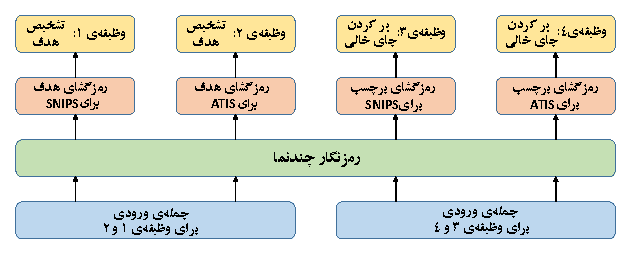
\includegraphics[scale=1.4]{Figures/federated.pdf}
	\caption[ساختار مدل \lr{Federated-Learning}]{ساختار مدل \lr{Federated-Learning} \cite{huang:2020}.}
	\label{Fig:federated}
\end{figure}


معماری \lr{Co-Interactive Transformer} \cite{Qin:2021} برای ادغام پیش زمینه‌ی تشخیص هدف و پر کردن جای خالی در یکدیگر معرفی شد و از مکانیزم توجه چند سر \cite{transformer} استفاده کرد. در \lr{Co-Interactive} به جای معماری رمزنگار - رمزگشا، معماری رمزنگار - ماژول تعاملی - رمزگشا معرفی شد. در رمزنگار، از یک \lr{LSTM‌} دوطرفه استفاده شد. سپس با استفاده از مکانیزم توجه \cite{attention_bahdanau}، برای تشخیص هدف و پر کردن جای خالی، به صورت جداگانه ماتریس توجه به دست آمد. در ماژول تعاملی پیشنهادی، از مکانیزم توجه چند سر \cite{transformer} استفاده شد؛ به این نحو که به ازای هر وظیفه‌ی، یک تبدیل خطی از ماتریس توجه آن وظیفه برای کلید، مقدار و پرسش ایجاد شد. سپس، ماتریس توجه برای هر وظیفه، با استفاده از کلید و مقدار همان وظیفه و پرسش وظیفه‌ی دیگر، محاسبه شد. بدین ترتیب در این ماژول، اطلاعات ماتریس توجه مربوط به هر دو وظیفه با یکدیگر ترکیب شد. در گام بعدی، مانند معماری ترنسفورمر، ماتریس ورودی با خروجی مکانیزم توجه توصیفی برای هر وظیفه، جمع و نرمالایز شد. در لایه‌ی تغذیه به جلو‌ی ماژول تعاملی، خروجی هرکدام از داده‌های نرمالایز شده مربوط به وظایف با یکدیگر الحاق شده و به یک لایه‌ی تغذیه به جلو داده می‌شود. حاصل خروجی این لایه‌ی تغذیه به جلو با خروجی لایه‌ی توجه تعاملی، جمع و نرمالایز شد. در پایان، برای رمزگشای پر کردن جای خالی از \lr{CRF}، و برای رمزگشای تشخیص هدف از \lr{Max-Pooling} استفاده شد.
\begin{figure}[!htb]
	\centering
	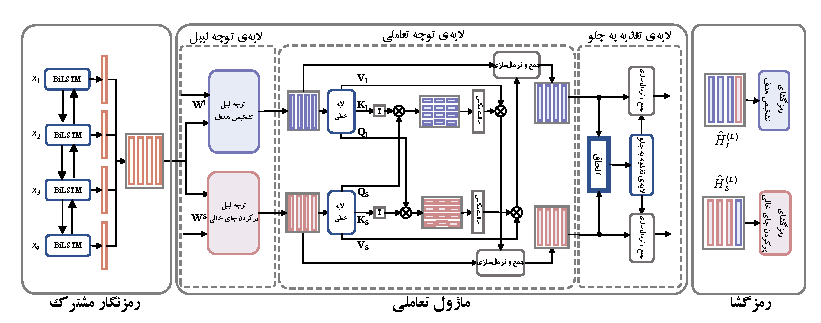
\includegraphics[scale=1.12]{Figures/cointeractive.pdf}
	\caption[ساختار مدل \lr{Co-Interactive Transformer}]{ساختار مدل \lr{Co-Interactive Transformer} \cite{Qin:2021}.}
	\label{Fig:cointeractive}
\end{figure}


در تلاشی دیگر برای ادغام بهینه‌ی دو وظیفه‌ی تشخیص هدف و پر کردن جای خالی، \lr{AISE} \cite{yang:2021} معرفی شد. معماری \lr{AISE}\LTRfootnote{Attending to Intent and Slots Explicitly} که در شکل \ref{Fig:aise} به تصویر کشیده شده، متشکل از یک رمزنگار مشترک، یک رمزنگار تشخیص هدف و مکانیزم پیشنهادی توجه چند سر پوشیده‌ی آگاه از موقعیت بود. مدل \lr{AISE} بر مبنای \lr{LSTM‌} و مکانیزم توجه چند سر بنا شد. در رمزگشای تشخیص هدف، از مکانیزم ادغام توجه چند سر استفاده کردند. ادغام توجه چند سر، نوعی از ادغام میانگین است که در آن وزن‌ها در میانگین گیری قابل تنظیم است. در این مکانیزم، کلید و مقدار از تعبیه‌ی رمزنگار و پرسش یک بردار، با مقادیر اولیه تصادفی و قابل آموزش است. خروجی این مکانیزم نیز، یک بردار با بعد تعبیه‌ی ورودی می‌باشد. در \lr{AISE}، برای رمزگشای پر کردن جای خالی، مکانیزم چند سر پوشیده‌ی آگاه از موقعیت معرفی شد. در مکانیزم پیشنهادی، از توجه چند سر پوشیده و برای تعبیه‌سازی ورودی نیز از تعبیه‌ی نسبی \cite{relative_positioning_transformer} استفاده شد. با توجه به اینکه خروجی‌های رمزگشای \lr{AISE} به صورت ترتیبی تولید شدند، در مکانیزم چند سر پوشیده، از تعبیه‌ی رمزنگار در موقعیت مربوط به نشانه‌ی درحال تولید به عنوان بردار پرسش استفاده می‌شد. همچنین از الحاق بردار زمینه‌ی تشخیص هدف و ماتریس تعبیه‌ی ابتدایی جمله به عنوان کلید و مقدار استفاده شد. در پایان، برچسب تولیدی در هر موقعیت، با استفاده از الحاق و سافت‌مکس بردار خروجی توجه چند سر پوشیده با بردار تعبیه‌ی مربوط به آن نشانه به دست آمد.
\begin{figure}[!htb]
	\centering
	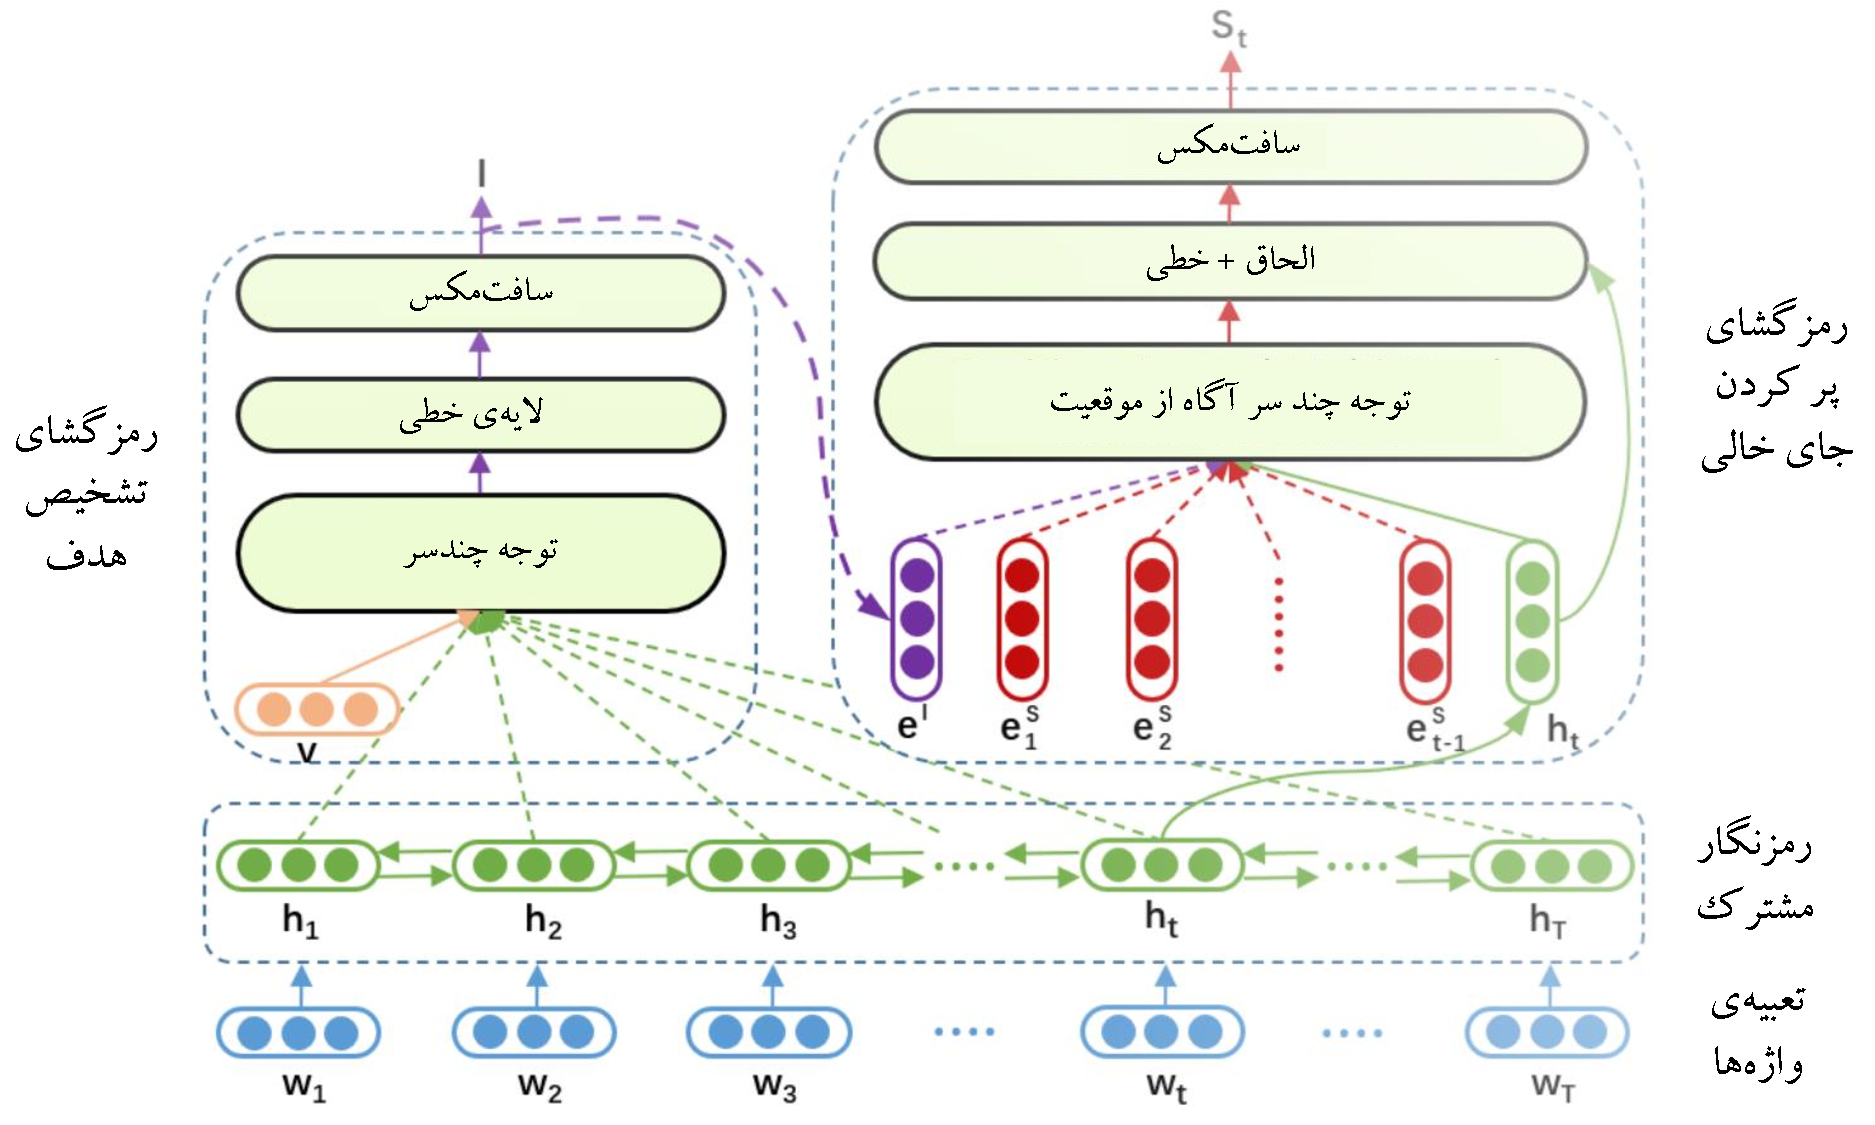
\includegraphics[scale=0.5]{Figures/aise.pdf}
	\caption[ساختار مدل \lr{AISE}]{ساختار مدل \lr{AISE} \cite{yang:2021}.}
	\label{Fig:aise}
\end{figure}


همچنین مدل پیشنهادی در \cite{Siddhant:2019} از المو به عنوان تعبیه‌ی اولیه، \lr{LSTM‌} دو طرفه به عنوان رمزنگار و \lr{CRF} به عنوان رمزگشا استفاده کرد. در این مقاله، به ارائه یک مدل زبانی تنظیم شده برای وظیفه‌ی برچسب زنی پرداخته شد و چند استراتژی برای سبک کردن مدل زبانی المو ارائه شد.
\section{جمع‌بندی}
در این فصل، انواع مدل‌های پیشین برای وظیفه‌ی درک زبان طبیعی ارائه شدند. از میان مدل‌های مبتنی بر تعبیه ثابت، \lr{Aligned LSTM} \cite{aligned_lstm_atten_nlu} با مکانیزم توجه، نخستین مدلی بود که اهمیت تراز بودن ورودی و خروجی را بیان کرد. سپس، مدل \lr{Aligned CNN-BLSTM} \cite{Wang:18} از ساختار لایه‌ی کانولوشنی-توالی ویژگی پنجره برای تعبیه‌ی ورودی خود استفاده کرد. مدل \lr{Slot-Gate} \cite{goo-etal-2018-slot} آموزش ضمنی دو وظیفه با یک رمزنگار مشترک را کافی نمی‌دانست؛ از این رو مکانیزمی برای کارگزاری هدف تشخیص داده شده در ورودی رمزگشای پر کردن جای خالی ارائه کرد. مدل \lr{Inter-Related} \cite{e:2019} این مکانیزم را یک طرفه دانست و مکانیزمی دو طرفه برای دخالت هر دو رمزگشا در یکدیگر ارائه کرد. همچنین، مدل \lr{PKJL} \cite{priorknowledge} برای دخالت دانش پیش‌زمینه در رمزگشا و مدل \lr{CharEmbed+GRU}‌ \cite{Firdaus:2021} برای ارائه یک تعبیه‌ی جدید معرفی گشتند. از طرف دیگر، در میان کارهایی که از مدل زبانی به عنوان رمزنگار استفاده کردند، برت و \lr{CRF} \cite{chen:2019} برای تولید برچسب استفاده شد. همچنین، \lr{SASGBC} \cite{Wang:2020} مکانیزم \lr{Slot-Gate} را پس از برت استفاده کرد. برخی از معماری‌های ارائه شده نیز مدل زبانی را به عنوان تعبیه‌ی کلمات استفاده کردند. در این میان، \lr{Federated Learning} \cite{huang:2020} رمزنگار چند نما و همچنین آموزش همزمان رمزنگار بر روی چند مجموعه داده را معرفی کرد. معماری \lr{Co-Interactive Transformer} \cite{Qin:2021} روشی جدید برای ادغام پیش زمینه‌ی تشخیص هدف و پر کردن جای خالی با استفاده از به اشتراک گذاری کلید و مقدار معرفی کرد. در پایان نیز، مدل \lr{AISE} \cite{yang:2021} شیوه‌ای جدید برای تولید برچسب، با استفاده از توجه چند سر آگاه از موقعیت ارائه کرد.





